\documentclass[border=10pt]{standalone}
\usepackage{tikz}
\usetikzlibrary{arrows.meta,positioning,shapes.geometric,calc,fit}
\usepackage{lmodern}
\usepackage[T1]{fontenc}
\usepackage{xcolor}

% Node type colors
\definecolor{epBlue}{HTML}{2563EB}
\definecolor{epFill}{HTML}{DBEAFE}
\definecolor{mwAmber}{HTML}{D97706}
\definecolor{mwFill}{HTML}{FEF3C7}
\definecolor{svcGreen}{HTML}{059669}
\definecolor{svcFill}{HTML}{D1FAE5}
\definecolor{daRed}{HTML}{DC2626}
\definecolor{daFill}{HTML}{FEE2E2}
\definecolor{edgeGray}{HTML}{6B7280}
\definecolor{borderGray}{HTML}{D1D5DB}

\begin{document}
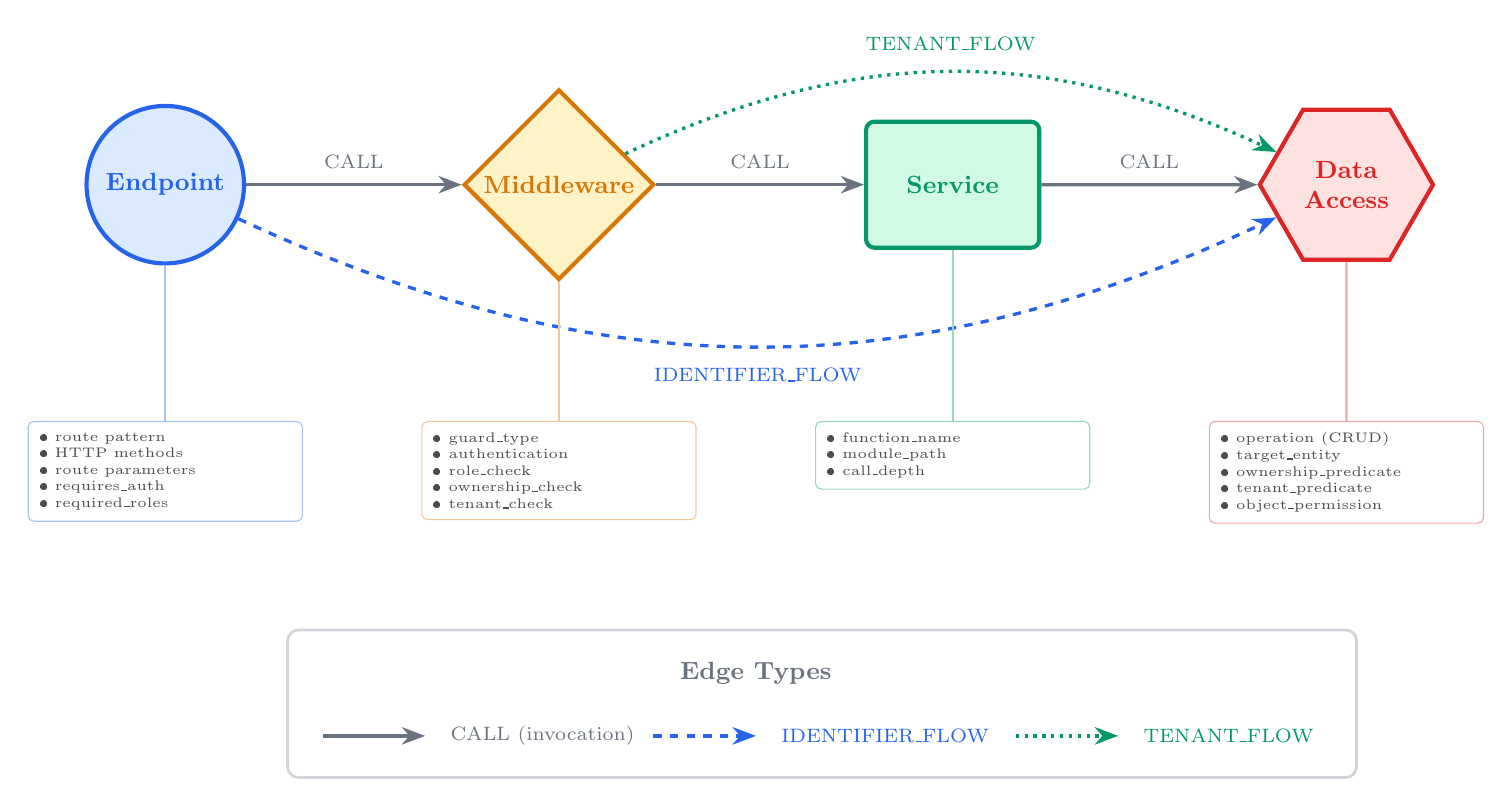
\begin{tikzpicture}[
    >=Stealth,
    every node/.style={font=\small},
    % Node shapes
    epnode/.style={
        circle, draw=epBlue, fill=epFill, line width=1.5pt,
        minimum size=2cm, align=center, font=\small\bfseries,
        text=epBlue
    },
    mwnode/.style={
        diamond, draw=mwAmber, fill=mwFill, line width=1.5pt,
        minimum size=2cm, align=center, font=\small\bfseries,
        text=mwAmber, inner sep=2pt
    },
    svcnode/.style={
        rectangle, draw=svcGreen, fill=svcFill, line width=1.5pt,
        minimum width=2.2cm, minimum height=1.6cm, align=center,
        font=\small\bfseries, text=svcGreen, rounded corners=3pt
    },
    danode/.style={
        regular polygon, regular polygon sides=6, draw=daRed, fill=daFill,
        line width=1.5pt, minimum size=2.2cm, align=center,
        font=\small\bfseries, text=daRed, inner sep=2pt
    },
    % Attribute box
    attrbox/.style={
        rectangle, rounded corners=2pt, draw=#1!40, fill=white,
        font=\tiny, text=black!70, align=left, inner sep=4pt
    },
    % Edge styles
    calledge/.style={->, line width=1.2pt, draw=edgeGray},
    idflowedge/.style={->, line width=1.2pt, draw=epBlue, dashed},
    tenantflowedge/.style={->, line width=1.2pt, draw=svcGreen, dotted},
]

% === Node types row (well spaced) ===
\node[epnode] (ep) at (0, 0) {Endpoint};
\node[mwnode] (mw) at (5, 0) {Middleware};
\node[svcnode] (svc) at (10, 0) {Service};
\node[danode] (da) at (15, 0) {Data\\Access};

% === Connecting arrows between nodes ===
\draw[calledge] (ep) -- node[above, font=\scriptsize, text=edgeGray, yshift=2pt] {CALL} (mw);
\draw[calledge] (mw) -- node[above, font=\scriptsize, text=edgeGray, yshift=2pt] {CALL} (svc);
\draw[calledge] (svc) -- node[above, font=\scriptsize, text=edgeGray, yshift=2pt] {CALL} (da);

% Identifier flow (curved, below)
\draw[idflowedge] (ep) to[bend right=25]
    node[below, font=\scriptsize, text=epBlue, yshift=-4pt] {IDENTIFIER\_FLOW} (da);

% Tenant flow (curved, above)
\draw[tenantflowedge] (mw) to[bend left=25]
    node[above, font=\scriptsize, text=svcGreen, yshift=4pt] {TENANT\_FLOW} (da);

% === Attribute boxes below each node (same level, lower) ===
\node[attrbox=epBlue, text width=3.2cm, anchor=north] (ep_attr) at (0, -3.0) {
    \textbullet\ route pattern\\
    \textbullet\ HTTP methods\\
    \textbullet\ route parameters\\
    \textbullet\ requires\_auth\\
    \textbullet\ required\_roles
};

\node[attrbox=mwAmber, text width=3.2cm, anchor=north] (mw_attr) at (5, -3.0) {
    \textbullet\ guard\_type\\
    \textbullet\ authentication\\
    \textbullet\ role\_check\\
    \textbullet\ ownership\_check\\
    \textbullet\ tenant\_check
};

\node[attrbox=svcGreen, text width=3.2cm, anchor=north] (svc_attr) at (10, -3.0) {
    \textbullet\ function\_name\\
    \textbullet\ module\_path\\
    \textbullet\ call\_depth
};

\node[attrbox=daRed, text width=3.2cm, anchor=north] (da_attr) at (15, -3.0) {
    \textbullet\ operation (CRUD)\\
    \textbullet\ target\_entity\\
    \textbullet\ ownership\_predicate\\
    \textbullet\ tenant\_predicate\\
    \textbullet\ object\_permission
};

% Connector lines from nodes to attribute boxes
\draw[draw=epBlue!40, line width=0.8pt] (ep.south) -- (ep_attr.north);
\draw[draw=mwAmber!40, line width=0.8pt] (mw.south) -- (mw_attr.north);
\draw[draw=svcGreen!40, line width=0.8pt] (svc.south) -- (svc_attr.north);
\draw[draw=daRed!40, line width=0.8pt] (da.south) -- (da_attr.north);

% === Edge legend inside a box ===
% Title
\node[font=\small\bfseries, text=edgeGray] (legend_title) at (7.5, -6.2) {Edge Types};

% Legend items — use coordinate nodes at arrow starts so fit includes them
\node[inner sep=0pt] (arr1_start) at (2.0, -7.0) {};
\draw[calledge] (2.0, -7.0) -- (3.3, -7.0);
\node[font=\scriptsize, anchor=west, text=edgeGray] (leg1) at (3.5, -7.0) {CALL (invocation)};

\draw[idflowedge] (6.2, -7.0) -- (7.5, -7.0);
\node[font=\scriptsize, anchor=west, text=epBlue] (leg2) at (7.7, -7.0) {IDENTIFIER\_FLOW};

\draw[tenantflowedge] (10.8, -7.0) -- (12.1, -7.0);
\node[font=\scriptsize, anchor=west, text=svcGreen] (leg3) at (12.3, -7.0) {TENANT\_FLOW};

% Box around legend (includes arrow start node)
\node[draw=borderGray, rounded corners=4pt, line width=1pt,
      inner xsep=12pt, inner ysep=8pt,
      fit=(legend_title)(arr1_start)(leg1)(leg2)(leg3)] {};

\end{tikzpicture}
\end{document}
